\documentclass[../main/thesis.tex]{subfiles}

\graphicspath{{/home/arefk/uio/MScThesis_AreKvanum2022_SeaIceML/thesis/datasets/figures/}}

\begin{document}
\section{Datasets}
The aim of this section is to perform a rundown of the different datasets used for the purpose of this thesis. This includes both internal datasets, in the sense that they are used for training the deep learning system, but also external datasets as in datasets only used for validating model performance. The term \textit{dataset} will for the scope of this thesis refer to a sequence of spatio-temporal structured arrays containing gridded values, and serves as a catch-all for model outputs and satellite products. 
 
\subsection{AROME Arctic}
A deep neural network can increase the skill of its predicitions by using correlated variables which provide additional information of the current state of Sea Ice. \todo{Dette må enten refreres til bakover i oppgaven eller siteres} For example, near surface winds influence the sea ice drift speed \cite{Spreen2011}, with the sea ice drift speed being inverse proportional to the sea ice concentration \cite{Yu2020}. Moreover, two meter temperature can also impact the growth of sea ice. AROME Arctic is a non-hydrostatic, convection resolving high-resolution weather forecasting system which covers the European Arctic \cite{Mueller2017}.


\subsection{Sea Ice Charts}
\todo{Få inn en figur som viser månedlig SIC fordeling fra Ice Chartsene, gjerne over en ti års periode. Som i \cite{Grigoryev2022}}

The Sea Ice charts is an operational Sea Ice Concentration product provided by MET Norway. The product is manually drawn by a Sea Ice Specialist, and is distributed every workday at 15:00 UTC. The Sea Ice specialist assesses available SAR data from Sentinel 1 and Radarsat 2. However, due to the spatial variability in daily SAR coverage, visual, infrared and low resolution passive microwave observations are supplied to achieve a consistent spatial coverage \cite{MOI2015}. The Sea Ice charts are drawn in an ArcGIS production environment, and is as such intrinsically not projected onto a defined grid. Yet, the operational product available for download on \href{https://resources.marine.copernicus.eu/product-detail/SEAICE_ARC_SEAICE_L4_NRT_OBSERVATIONS_011_002/INFORMATION}{Copernicus} is provided as mean values on a 1km grid.

From the description of the Sea Ice charts given above, it is worth addressing the spatial inconsistency following the projection onto a uniformly sized grid. As the Sea Ice specialist draws polygons based on data from different satellite sources with a wide range of spatial resolution (80m from SAR, 1000m from visible / infrared and even lower resolution for passive microwave), the underlying uncertainty and detailed structures in the Sea Ice chart varies \cite{MOI2015}. Furthermore, I was made aware by one of the Sea Ice Analysts that time constraints also limits the hours different sections of the Ice chart is alloted. Moreover, the Sea Ice charts is an operational product aimed at end users in industries such as fishing, tourism, shipping or other maritime operations. This influences the decision-making when creating the final operational product. \todo{ask Trond on email}. As a consequence, the Sea Ice analyst spends approximately half of the total time draw polygons around the Svalbard archipelago. 

In conclusion, concerning the limited resources available both with regards to data availability as well as total hours available, the Sea Ice charts represents a dataset with a spatial uncertainty that is non-uniform across a single sample, and that changes in time. In spite of that, the involvement of a Sea Ice specialist which manually assures each Sea Ice charts, the temporal consistency as well as their high resolution has led us to believe that the Sea Ice charts is the overall best Sea Ice Concentration product available for the current study region.

\begin{figure}
    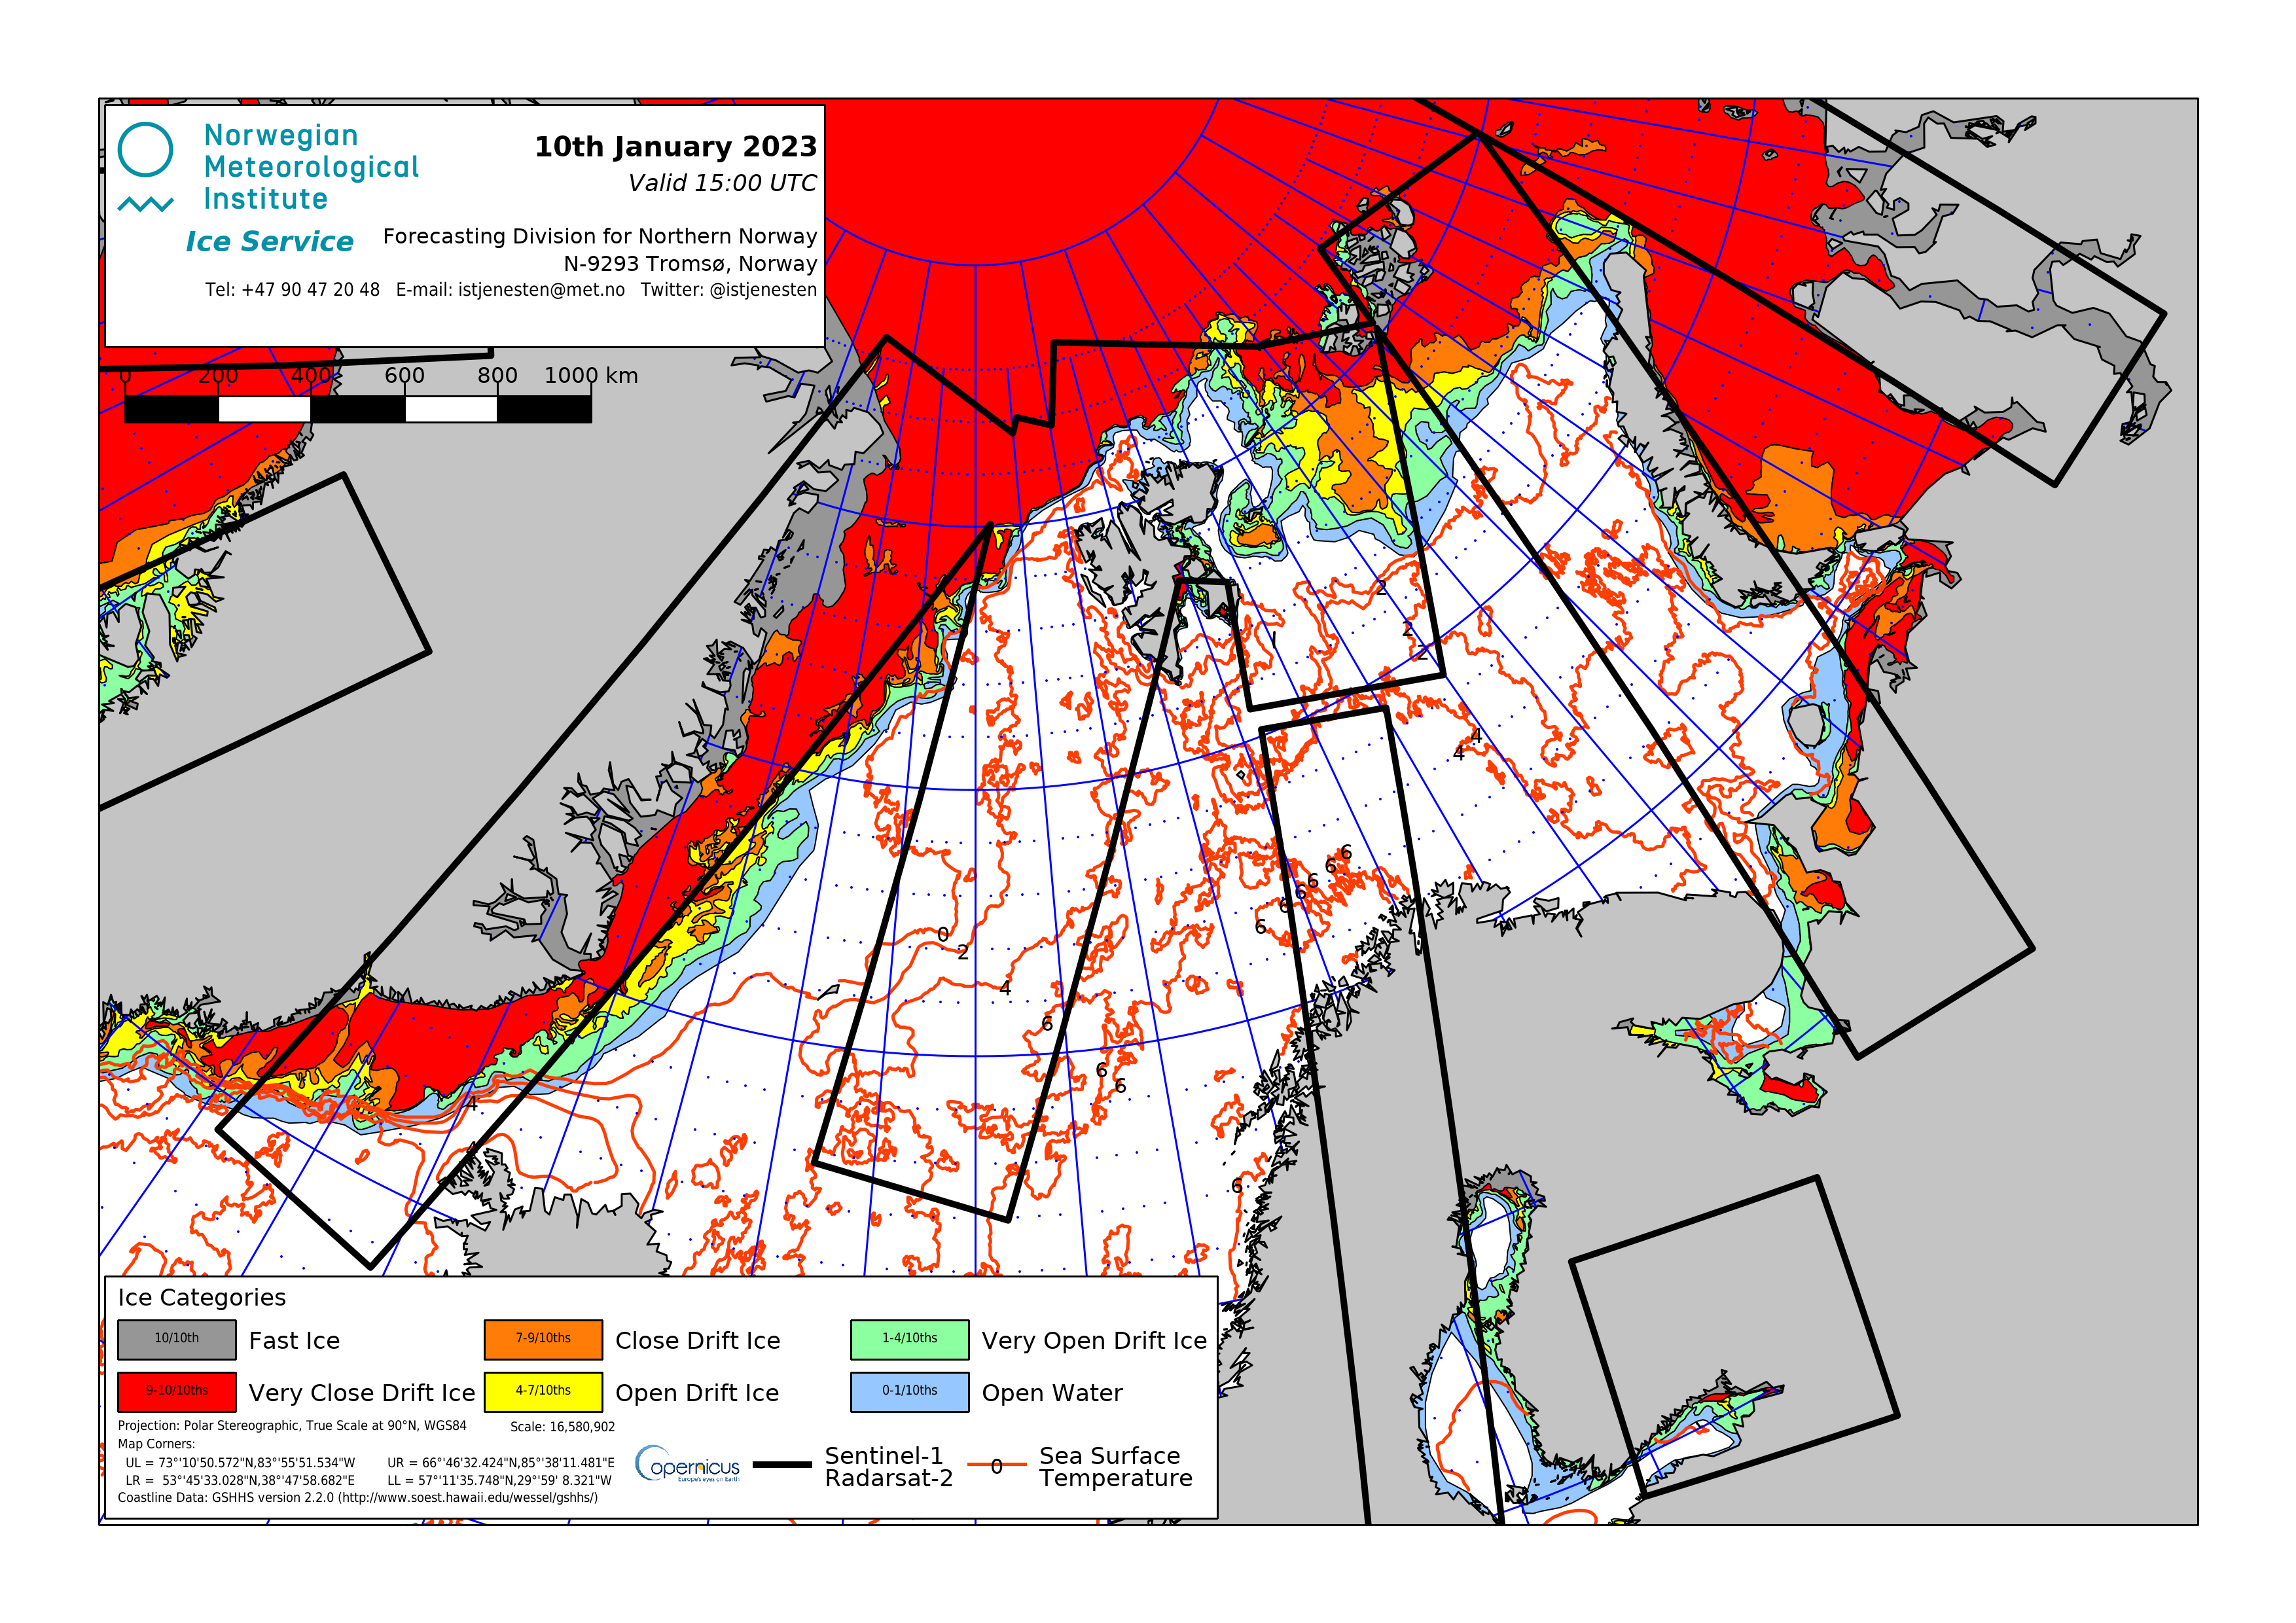
\includegraphics[width=\textwidth]{general_latest}
\end{figure}

\subsection{Osi-Saf}
\todo{Mention how when using Osi Saf trend as predictor, the trend up to but not including the forecast start date is used. This is to make the model ready for operational use, as the Osi Saf daily product is not ready on lustre when the Ice Charts are poublished at UTC 15:00}

\subsection{AMSR2}

\subsection{NeXtSIM}
The NeXtSIM-f forecasting system uses a standalone sea ice model (NeXtSIM), and is not coupled with an ocean model \cite{Williams2021}. Furthermore, NeXtSIM differentiates itself from comparative physical sea ice models as it does not apply a rheology based on the Viscous-Plastic scheme. Note that the rheology of a sea ice model refers to how the model relates ice deformation and ice thickness with the internal stresses in the ice \cite{Hibler1979}. internal stress. Instead, NeXtSIM applies a brittle sea ice rheology, specifically the Maxwell elasto-brittle rheology which treats the sea ice as a brittle material rather than a viscous fluid \cite{Dansereau2016}.



\subsection{Barents-2.5}
Barents-2.5 is an in-development operational coupled ocean and sea ice forecasting model at MET Norway \cite{Roehrs2022}. The model has been in operation since September 2021. Barents-2.5 poses the same resolution and projection as AA, i.e. Lambert Conformal Conic with a 2.5 kilometer resolution \cite{Roehrs2022,Mueller2017}. The sea ice model used in Barents-2.5 is the Los Alamos sea ice model (CICE) version 5.1, which uses an Elastic Viscous Plastic sea ice Rheology \cite{Hunke2015}. Thus, the CICE model represents sea ice as a viscous fluid which creeps slowly given small stresses and deforms plastically under large stress. It is also noted that the elastic behavior was introduced to benefit the numerical aspects of the model, and can be considered unrealistic from a physical point of view \cite{Hunke1997}.

As part of the forcing routine, Barents-2.5 performs non-homogenous atmospheric forcing of its ensemble members, with one member of each ensemble being forced with AA while the rest of the members is forces using atmospheric data from ECMWF. As such, the member forced with AA seem to perform best with regards to ocean currents, but the atmospheric forcing's impact on SIC performance is unknown at the time of writing. However, there is generally little ensemble spread with regards to sea ice (Johannes Röhrs, 2022, pers. commun.)

The data assimilation scheme applied for Barents-2.5 is a Deterministic Ensemble Kalman filter, which solves for the analysis though with a background error covariance matrix estimated as the variance of the ensemble of background members \cite{Roehrs2022}. Furthermore, it has been expressed by the developers of the model that the model performance was unsatisfactory up until May / June 2022 due to spin up time of the data assimilation system (ohannes Röhrs, 2022, pers. commun.). This coincides with the formulation of the Ensemble Kalman filter as a Monte Carlo formulation of the Kalman filter \cite{Sakov2008}. Hence, it is expected that the data assimilation scheme used in Barents-2.5 improves the forecasts over time.





% Local bibliography
\biblio

\end{document}